% Options for packages loaded elsewhere
% Options for packages loaded elsewhere
\PassOptionsToPackage{unicode}{hyperref}
\PassOptionsToPackage{hyphens}{url}
%
\documentclass[
  english,
  russian,
  12pt,
  a4paper,
  DIV=11,
  numbers=noendperiod]{scrreprt}
\usepackage{xcolor}
\usepackage{amsmath,amssymb}
\setcounter{secnumdepth}{5}
\usepackage{iftex}
\ifPDFTeX
  \usepackage[T1]{fontenc}
  \usepackage[utf8]{inputenc}
  \usepackage{textcomp} % provide euro and other symbols
\else % if luatex or xetex
  \usepackage{unicode-math} % this also loads fontspec
  \defaultfontfeatures{Scale=MatchLowercase}
  \defaultfontfeatures[\rmfamily]{Ligatures=TeX,Scale=1}
\fi
\usepackage{lmodern}
\ifPDFTeX\else
  % xetex/luatex font selection
\fi
% Use upquote if available, for straight quotes in verbatim environments
\IfFileExists{upquote.sty}{\usepackage{upquote}}{}
\IfFileExists{microtype.sty}{% use microtype if available
  \usepackage[]{microtype}
  \UseMicrotypeSet[protrusion]{basicmath} % disable protrusion for tt fonts
}{}
\usepackage{setspace}
% Make \paragraph and \subparagraph free-standing
\makeatletter
\ifx\paragraph\undefined\else
  \let\oldparagraph\paragraph
  \renewcommand{\paragraph}{
    \@ifstar
      \xxxParagraphStar
      \xxxParagraphNoStar
  }
  \newcommand{\xxxParagraphStar}[1]{\oldparagraph*{#1}\mbox{}}
  \newcommand{\xxxParagraphNoStar}[1]{\oldparagraph{#1}\mbox{}}
\fi
\ifx\subparagraph\undefined\else
  \let\oldsubparagraph\subparagraph
  \renewcommand{\subparagraph}{
    \@ifstar
      \xxxSubParagraphStar
      \xxxSubParagraphNoStar
  }
  \newcommand{\xxxSubParagraphStar}[1]{\oldsubparagraph*{#1}\mbox{}}
  \newcommand{\xxxSubParagraphNoStar}[1]{\oldsubparagraph{#1}\mbox{}}
\fi
\makeatother


\usepackage{longtable,booktabs,array}
\usepackage{calc} % for calculating minipage widths
% Correct order of tables after \paragraph or \subparagraph
\usepackage{etoolbox}
\makeatletter
\patchcmd\longtable{\par}{\if@noskipsec\mbox{}\fi\par}{}{}
\makeatother
% Allow footnotes in longtable head/foot
\IfFileExists{footnotehyper.sty}{\usepackage{footnotehyper}}{\usepackage{footnote}}
\makesavenoteenv{longtable}
\usepackage{graphicx}
\makeatletter
\newsavebox\pandoc@box
\newcommand*\pandocbounded[1]{% scales image to fit in text height/width
  \sbox\pandoc@box{#1}%
  \Gscale@div\@tempa{\textheight}{\dimexpr\ht\pandoc@box+\dp\pandoc@box\relax}%
  \Gscale@div\@tempb{\linewidth}{\wd\pandoc@box}%
  \ifdim\@tempb\p@<\@tempa\p@\let\@tempa\@tempb\fi% select the smaller of both
  \ifdim\@tempa\p@<\p@\scalebox{\@tempa}{\usebox\pandoc@box}%
  \else\usebox{\pandoc@box}%
  \fi%
}
% Set default figure placement to htbp
\def\fps@figure{htbp}
\makeatother



\ifLuaTeX
\usepackage[bidi=basic,provide=*]{babel}
\else
\usepackage[bidi=default,provide=*]{babel}
\fi
% get rid of language-specific shorthands (see #6817):
\let\LanguageShortHands\languageshorthands
\def\languageshorthands#1{}


\setlength{\emergencystretch}{3em} % prevent overfull lines

\providecommand{\tightlist}{%
  \setlength{\itemsep}{0pt}\setlength{\parskip}{0pt}}



 
\usepackage[style=gost-numeric,backend=biber,langhook=extras,autolang=other*]{biblatex}
\addbibresource{bib/cite.bib}

\usepackage[]{csquotes}

\usepackage{indentfirst}
\usepackage{float}
\floatplacement{figure}{H}
\IfFileExists{plex-otf.sty}{
  %% Full TeXlive
  \usepackage[
    % math,
    RM={Scale=0.94},SS={Scale=0.94},SScon={Scale=0.94},TT={Scale=MatchLowercase,FakeStretch=0.9},
    DefaultFeatures={Ligatures=Common}
  ]{plex-otf}
  % \usepackage[Scale=MatchUppercase]{juliamono}
}{
  %% TinyTeX
  \usepackage{libertine}
}
\KOMAoption{captions}{tableheading}
\makeatletter
\@ifpackageloaded{caption}{}{\usepackage{caption}}
\AtBeginDocument{%
\ifdefined\contentsname
  \renewcommand*\contentsname{Содержание}
\else
  \newcommand\contentsname{Содержание}
\fi
\ifdefined\listfigurename
  \renewcommand*\listfigurename{Список иллюстраций}
\else
  \newcommand\listfigurename{Список иллюстраций}
\fi
\ifdefined\listtablename
  \renewcommand*\listtablename{Список таблиц}
\else
  \newcommand\listtablename{Список таблиц}
\fi
\ifdefined\figurename
  \renewcommand*\figurename{Рисунок}
\else
  \newcommand\figurename{Рисунок}
\fi
\ifdefined\tablename
  \renewcommand*\tablename{Таблица}
\else
  \newcommand\tablename{Таблица}
\fi
}
\@ifpackageloaded{float}{}{\usepackage{float}}
\floatstyle{ruled}
\@ifundefined{c@chapter}{\newfloat{codelisting}{h}{lop}}{\newfloat{codelisting}{h}{lop}[chapter]}
\floatname{codelisting}{Список}
\newcommand*\listoflistings{\listof{codelisting}{Листинги}}
\makeatother
\makeatletter
\makeatother
\makeatletter
\@ifpackageloaded{caption}{}{\usepackage{caption}}
\@ifpackageloaded{subcaption}{}{\usepackage{subcaption}}
\makeatother
\usepackage{bookmark}
\IfFileExists{xurl.sty}{\usepackage{xurl}}{} % add URL line breaks if available
\urlstyle{same}
\hypersetup{
  pdftitle={Отчёт по лабораторной работе №1},
  pdfauthor={Алексей С. Прядко},
  pdflang={ru-RU},
  hidelinks,
  pdfcreator={LaTeX via pandoc}}


\title{Отчёт по лабораторной работе №1}
\usepackage{etoolbox}
\makeatletter
\providecommand{\subtitle}[1]{% add subtitle to \maketitle
  \apptocmd{\@title}{\par {\large #1 \par}}{}{}
}
\makeatother
\subtitle{Установка и конфигурация операционной системы на виртуальную
машину}
\author{Алексей С. Прядко}
\date{}
\begin{document}
\maketitle

\renewcommand*\contentsname{Содержание}
{
\setcounter{tocdepth}{1}
\tableofcontents
}
\listoffigures
\listoftables

\setstretch{1.5}
\chapter{Цель
работы}\label{ux446ux435ux43bux44c-ux440ux430ux431ux43eux442ux44b}

Приобретение практических навыков установки операционной системы на
виртуальную машину, настройки минимально необходимых для дальнейшей
работы сервисов.

Цель данного отчёта --- зафиксировать процесс развёртывания ОС Rocky
Linux 8.10 и продемонстрировать владение базовыми инструментами анализа
системы.

\chapter{Задание}\label{ux437ux430ux434ux430ux43dux438ux435}

\begin{enumerate}
\def\labelenumi{\arabic{enumi}.}
\tightlist
\item
  Создать виртуальную машину с именем \texttt{aspryadko}.
\item
  Установить ОС Rocky Linux 8.10.
\item
  Собрать информацию о системе (ядро, процессор, память, файловая
  система).
\end{enumerate}

\chapter{Теоретическое
введение}\label{ux442ux435ux43eux440ux435ux442ux438ux447ux435ux441ux43aux43eux435-ux432ux432ux435ux434ux435ux43dux438ux435}

В рамках данной работы производится установка дистрибутива Rocky Linux,
который является бинарно совместимым с Red Hat Enterprise Linux (RHEL).
Для управления ресурсами используется гипервизор (VirtualBox),
позволяющий изолировать гостевую ОС от хостовой. Основные сведения о
системе в Linux-системах традиционно извлекаются из виртуальной файловой
системы \texttt{/proc} или с помощью специализированных утилит типа
\texttt{hostnamectl} и \texttt{df}.

\chapter{Выполнение лабораторной
работы}\label{ux432ux44bux43fux43eux43bux43dux435ux43dux438ux435-ux43bux430ux431ux43eux440ux430ux442ux43eux440ux43dux43eux439-ux440ux430ux431ux43eux442ux44b}

\section{Установка
ОС}\label{ux443ux441ux442ux430ux43dux43eux432ux43aux430-ux43eux441}

В процессе работы была создана виртуальная машина со следующими
параметрами: * \textbf{Имя:} aspryadko * \textbf{ОС:} Red Hat (64-bit) *
\textbf{Память:} 4096 MB * \textbf{Диск:} 40 GB

При установке было задано имя хоста \texttt{aspryadko.localdomain} и
создан пользователь \texttt{aspryadko} с правами администратора.

\section{Сбор сведений о
системе}\label{ux441ux431ux43eux440-ux441ux432ux435ux434ux435ux43dux438ux439-ux43e-ux441ux438ux441ux442ux435ux43cux435}

Ниже представлены результаты выполнения команд для анализа конфигурации
установленной системы.

\begin{enumerate}
\def\labelenumi{\arabic{enumi}.}
\tightlist
\item
  \textbf{Версия ядра Linux.} Использована команда \texttt{hostnamectl}
  (рис. Рисунок~\ref{fig-001}).
\end{enumerate}

\begin{figure}

\centering{

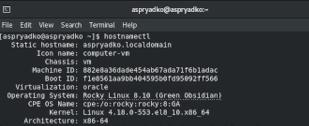
\includegraphics[width=0.7\linewidth,height=\textheight,keepaspectratio]{image/host.png}

}

\caption{\label{fig-001}Сведения о хосте и ядре}

\end{figure}%

\begin{enumerate}
\def\labelenumi{\arabic{enumi}.}
\setcounter{enumi}{1}
\tightlist
\item
  \textbf{Частота процессора (Detected Mhz).} Данные извлечены из
  системного файла \texttt{/proc/cpuinfo} (рис. Рисунок~\ref{fig-002}).
\end{enumerate}

\begin{figure}

\centering{

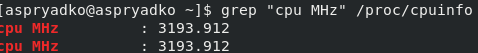
\includegraphics[width=0.7\linewidth,height=\textheight,keepaspectratio]{image/cpu_mhz.png}

}

\caption{\label{fig-002}Частота процессора}

\end{figure}%

\begin{enumerate}
\def\labelenumi{\arabic{enumi}.}
\setcounter{enumi}{2}
\tightlist
\item
  \textbf{Модель процессора.} Использован вывод из того же файла (рис.
  Рисунок~\ref{fig-003}).
\end{enumerate}

\begin{figure}

\centering{

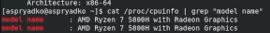
\includegraphics[width=0.7\linewidth,height=\textheight,keepaspectratio]{image/cpu.png}

}

\caption{\label{fig-003}Модель процессора}

\end{figure}%

\begin{enumerate}
\def\labelenumi{\arabic{enumi}.}
\setcounter{enumi}{3}
\tightlist
\item
  \textbf{Объем оперативной памяти.} Использована команда
  \texttt{free\ -m} (рис. Рисунок~\ref{fig-004}).
\end{enumerate}

\begin{figure}

\centering{

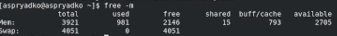
\includegraphics[width=0.7\linewidth,height=\textheight,keepaspectratio]{image/mem.png}

}

\caption{\label{fig-004}Оперативная память}

\end{figure}%

\begin{enumerate}
\def\labelenumi{\arabic{enumi}.}
\setcounter{enumi}{4}
\tightlist
\item
  \textbf{Тип файловой системы.} Использована команда \texttt{df\ -Th}
  (рис. Рисунок~\ref{fig-005}).
\end{enumerate}

\begin{figure}

\centering{

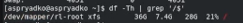
\includegraphics[width=0.7\linewidth,height=\textheight,keepaspectratio]{image/fs.png}

}

\caption{\label{fig-005}Файловая система}

\end{figure}%

\begin{enumerate}
\def\labelenumi{\arabic{enumi}.}
\setcounter{enumi}{5}
\tightlist
\item
  \textbf{Тип гипервизора.} Использована команда \texttt{virt-what}
  (рис. Рисунок~\ref{fig-006}).
\end{enumerate}

\begin{figure}

\centering{

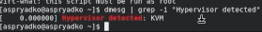
\includegraphics[width=0.7\linewidth,height=\textheight,keepaspectratio]{image/virt.png}

}

\caption{\label{fig-006}Тип гипервизора}

\end{figure}%

\begin{enumerate}
\def\labelenumi{\arabic{enumi}.}
\setcounter{enumi}{6}
\tightlist
\item
  \textbf{Последовательность монтирования файловых систем.} Получена с
  помощью команды \texttt{findmnt} (рис. Рисунок~\ref{fig-007}).
\end{enumerate}

\begin{figure}

\centering{

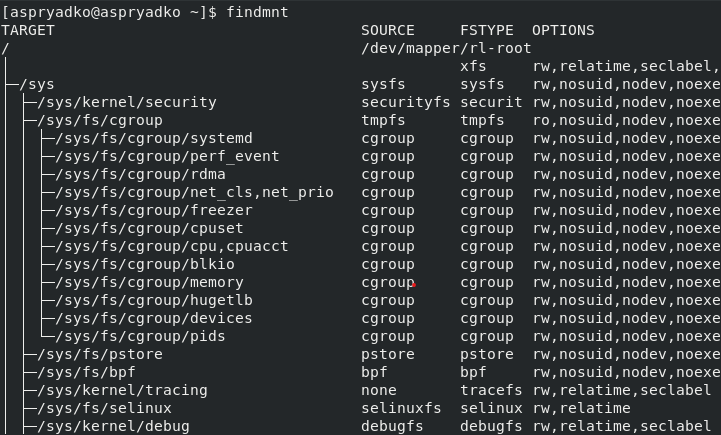
\includegraphics[width=0.7\linewidth,height=\textheight,keepaspectratio]{image/mount_seq.png}

}

\caption{\label{fig-007}Последовательность монтирования}

\end{figure}%

\chapter{Ответы на контрольные
вопросы}\label{ux43eux442ux432ux435ux442ux44b-ux43dux430-ux43aux43eux43dux442ux440ux43eux43bux44cux43dux44bux435-ux432ux43eux43fux440ux43eux441ux44b}

\begin{enumerate}
\def\labelenumi{\arabic{enumi}.}
\item
  \textbf{Какую информацию содержит учётная запись пользователя?}
  Учётная запись (хранится в \texttt{/etc/passwd} и
  \texttt{/etc/shadow}) включает: логин, UID и GID, полное имя, домашний
  каталог, командную оболочку и хеш пароля.
\item
  \textbf{Команды терминала:}

  \begin{itemize}
  \tightlist
  \item
    \textbf{Справка:} \texttt{man\ \textless{}команда\textgreater{}},
    \texttt{\textless{}команда\textgreater{}\ -\/-help}.
  \item
    \textbf{Навигация:} \texttt{cd\ \textless{}путь\textgreater{}}.
  \item
    \textbf{Просмотр каталога:} \texttt{ls\ -la}.
  \item
    \textbf{Объём папки:}
    \texttt{du\ -sh\ \textless{}путь\textgreater{}}.
  \item
    \textbf{Манипуляции с файлами:} \texttt{mkdir} (каталог),
    \texttt{touch} (файл), \texttt{rm} (удаление).
  \item
    \textbf{Права доступа:} \texttt{chmod}.
  \item
    \textbf{История:} \texttt{history}.
  \end{itemize}
\item
  \textbf{Что такое файловая система?} Это способ организации данных.
  Примеры: \textbf{XFS} (высокая производительность), \textbf{Ext4}
  (стандарт Linux), \textbf{NTFS} (стандарт Windows).
\item
  \textbf{Как посмотреть смонтированные ФС?} Команды \texttt{mount}
  (подробно) и \texttt{df\ -Th} (удобно для чтения).
\item
  \textbf{Как удалить зависший процесс?} Узнать PID через \texttt{top}
  или \texttt{ps}, затем выполнить
  \texttt{kill\ \textless{}PID\textgreater{}} или
  \texttt{kill\ -9\ \textless{}PID\textgreater{}} для принудительного
  завершения.
\end{enumerate}

\chapter{Выводы}\label{ux432ux44bux432ux43eux434ux44b}

В ходе выполнения лабораторной работы я научился создавать виртуальные
машины в среде VirtualBox, устанавливать операционную систему семейства
Linux (на примере Rocky Linux) и использовать базовый инструментарий
терминала для анализа аппаратных и программных характеристик системы.

\chapter*{Список
литературы}\label{ux441ux43fux438ux441ux43eux43a-ux43bux438ux442ux435ux440ux430ux442ux443ux440ux44b}
\addcontentsline{toc}{chapter}{Список литературы}

\printbibliography[heading=none]





\end{document}
